%%%%%%%%%%%%%%%%%%%%%%%%%%%%%%%%%%%%%%%%%%%%%%%%%%%%%%%%%%%%%%%%%%%%%%%%%%%%%%%%%%
\begin{frame}[fragile]\frametitle{}
\begin{center}
{\Large Will AI Replace Teachers?}
\end{center}
\end{frame}

%%%%%%%%%%%%%%%%%%%%%%%%%%%%%%%%%%%%%%%%%%%%%%%%%%%
\begin{frame}[fragile]\frametitle{The Fear Behind Every AI Wave}
\begin{itemize}
\item Every major AI advance since the 1980s has come with the same headline: ``this job is over.''
\item Radiology got there first, and loudest, a full decade before ChatGPT existed.
\item What actually happened to that profession is the single most useful data point we have for thinking about teaching.
\end{itemize}
\end{frame}

%%%%%%%%%%%%%%%%%%%%%%%%%%%%%%%%%%%%%%%%%%%%%%%%%%%
\begin{frame}[fragile]\frametitle{2016: A Very Confident Prediction}
\begin{itemize}
\item Geoffrey Hinton, the ``Godfather of AI'' and a Nobel laureate, told a room of doctors in 2016:
\end{itemize}
\begin{alertblock}{Hinton, 2016}
``We should stop training radiologists now. It's just completely obvious that within five years, deep learning is going to do better than radiologists.''
\end{alertblock}
\begin{itemize}
\item He later said, to the New York Times, that he had spoken too broadly.
\end{itemize}
{\tiny (Ref: New York Times, revisited in \emph{radiologybusiness.com}, 2026.)}
\end{frame}

%%%%%%%%%%%%%%%%%%%%%%%%%%%%%%%%%%%%%%%%%%%%%%%%%%%
\begin{frame}[fragile]\frametitle{2026: What Actually Happened}
\begin{itemize}
\item Radiologist headcount grew \textbf{12\%} from 2010 to 2022 (Journal of the American College of Radiology).
\item Demand for radiologists \textbf{tripled} between 2016 and 2022, the exact window Hinton's five years covered.
\item The workforce is projected to grow another \textbf{26--40\%} by 2055.
\item Salaries: up to \$571K, and still climbing.
\end{itemize}
{\tiny (Refs: JACR workforce studies; Fortune, ``A decade after the Godfather of AI said radiologists were obsolete'', 2026.)}
\end{frame}

%%%%%%%%%%%%%%%%%%%%%%%%%%%%%%%%%%%%%%%%%%%%%%%%%%%
\begin{frame}[fragile]\frametitle{Why the Prediction Failed: Tasks, Not Jobs}

\adjustbox{valign=t}{%
\begin{minipage}{0.55\linewidth}
\begin{itemize}
\item ``Radiologist'' is not one task, it is a bundle of roughly \textbf{27 distinct tasks}.
\item Reading a scan is one of them. AI got very good at exactly that one.
\item The other 26, consulting with physicians, explaining findings to a scared patient, deciding what to biopsy, performing image-guided procedures, did not go anywhere.
\item A job survives as long as most of its tasks resist automation, even when one high-profile task falls.
\end{itemize}
\end{minipage}%
}%
\hfill%
\adjustbox{valign=t}{%
\begin{minipage}{0.4\linewidth}
\begin{center}
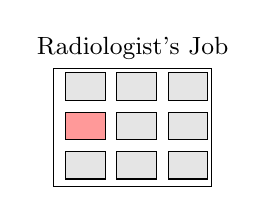
\begin{tikzpicture}[scale=0.5]
\draw (0,0) rectangle (4,3);
\node[above] at (2,3) {\small Radiologist's Job};
\foreach \x/\y/\c/\lbl in {0.3/2.2/gray!20/consult, 1.6/2.2/gray!20/plan,
  2.9/2.2/gray!20/procedure, 0.3/1.2/red!40/{\bf read}, 1.6/1.2/gray!20/report,
  2.9/1.2/gray!20/mentor, 0.3/0.2/gray!20/explain, 1.6/0.2/gray!20/sedate,
  2.9/0.2/gray!20/{\ldots}}{
  \draw[fill=\c] (\x,\y) rectangle ++(1,0.7);
}
\end{tikzpicture}
\end{center}
{\tiny One shaded task (image reading) got automated. The other $\sim$26 did not.}
\end{minipage}%
}
\end{frame}

%%%%%%%%%%%%%%%%%%%%%%%%%%%%%%%%%%%%%%%%%%%%%%%%%%%
\begin{frame}[fragile]\frametitle{The Same Logic Applies to Teaching}
\begin{itemize}
\item ``Teacher'' is also a bundle of tasks, not one thing.
\item \textbf{Highly automatable:} drafting a first-pass lesson outline, generating quiz questions, summarizing 50 feedback forms, writing a first draft of report comments.
\item \textbf{Not automatable any time soon:} noticing a student is struggling before they say so, managing a room of 30 restless 12-year-olds, a difficult conversation with a parent, being the adult a kid trusts.
\item AI is quietly eating the first list. Nobody is close to touching the second.
\end{itemize}
\end{frame}

%%%%%%%%%%%%%%%%%%%%%%%%%%%%%%%%%%%%%%%%%%%%%%%%%%%
\begin{frame}[fragile]\frametitle{Quick Check: Task or Job?}
\begin{itemize}
\item Nvidia's CEO Jensen Huang put it this way in 2026: \emph{``AI kills tasks, not jobs.''}
\item For each of these, is AI automating a \textbf{task} within teaching, or threatening the \textbf{job} of teaching itself?
\begin{itemize}
\item Grading 40 multiple-choice quizzes
\item Resolving a conflict between two students at recess
\item Drafting a first pass at a rubric
\item Deciding whether a struggling student needs extra support
\end{itemize}
\end{itemize}
\end{frame}

%%%%%%%%%%%%%%%%%%%%%%%%%%%%%%%%%%%%%%%%%%%%%%%%%%%
\begin{frame}[fragile]\frametitle{Quick Check: Answer}
\begin{itemize}
\item Grading MCQs, drafting a rubric: \textbf{tasks}. Mechanical, pattern-based, already being automated, and that is fine.
\item Resolving a peer conflict, judging who needs support: \textbf{the job}. These need judgment, context, and a relationship built over months, exactly what nobody has figured out how to automate.
\item \textbf{The reframe:} the question is never ``will AI replace teachers,'' it is ``which specific tasks on my plate can I hand off this term.''
\end{itemize}
\end{frame}
